\documentclass{article}
\usepackage{amsmath} 
\usepackage{graphicx} 
\usepackage{authblk}
\usepackage{url}
\usepackage{hyperref}
\usepackage{multirow}
\usepackage{amssymb}
\usepackage[linesnumbered,boxed]{algorithm2e}

\topmargin 0.0cm
\oddsidemargin 0.2cm
\textwidth 16cm 
\textheight 21cm
\footskip 1.0cm

\title{Numerical Method for Eigenvalue Problem and Its Application in Physics}
\author[1]{Mengzhi Chen}
\author[1]{Tong Li}
\affil[1]{Department of Physics and Astronomy, Michigan State University}
\date{}

\begin{document}
	\maketitle
	\begin{abstract}\label{abstract}
Eigenvalue decomposition of a Hermitian (or real symmetric) matrix is often the last step to solve a physics problem, and thus 
in this report we investigate different numerical methods for the eigenvalue problem. 
First two examples, buckling beam problem and quantum dot, are given to illustrate how a differential equation is transformed 
to an eigenvalue problem of a real symmetric matrix. 
Then we discuss details of Jacobi's and bisection methods, two important numerical algorithms for the eigenvalue problem. 
Applications of these two methods on the quantum dot are studied, which shows us when our approximation is good. 
In addition, we find that bisection method has a better performance and accuracy than Jacobi's. 
Therefore, bisection algorithm is usually more appropriate to utilize in physics. 
	\end{abstract}

	\section{Introduction}\label{intro}
Eigenvalue problem is an important mathematical problem that appears commonly in science and engineering. 
For matrix $A\in\mathbb{C}^{n \times n}$, its eigenvalues $\lambda_i$ and corresponding eigenvectors $\mathbf{v}_i\in\mathbb{C}^n$ satisfy
\begin{equation}
A\mathbf{v}_i=\lambda_i \mathbf{v}_i\ .
\end{equation}
If $A$ is Hermitian (or real symmetric), we can use its eigenvalues and eigenvectors to construct a unitary (or orthogonal) 
similarity transformation to diagonalize $A$, i.e. 
\begin{eqnarray}
S^{\dagger}AS=\text{diag}\{\lambda_1,\lambda_2,\cdots,\lambda_n\}\text{ for Hermitian }A\in\mathbb{C}^{n\times n}, \\
S^{T}AS=\text{diag}\{\lambda_1,\lambda_2,\cdots,\lambda_n\}\text{ for symmetric }A\in\mathbb{R}^{n\times n},
\end{eqnarray}
where $S$ is a unitary (or orthogonal) matrix and the $i$th column of $S$ is the eigenvector of $A$ with eigenvalue $\lambda_i$. 
\par
The diagonalization of a Hermitian (or real symmetric) matrix is usually the final step of a physics problem. 
In Sec. \ref{physcis_problem} we give two examples of eigenvalue problems in physics, which shows how a differential equation 
is transformed to an eigenvalue problem of a real symmetric matrix. 
We introduce two algorithms, Jacobi's methods and bisection method in Sec. \ref{method}, to solve the eigenvalue problem. 
In Sec. \ref{results} our numerical solutions are compared with the analytical solution 
to show under what condition our approximation is valid. 
We also discuss the performance of the two algorithms we implement in Sec. \ref{results}. 
Conclusions and outlook are given in Sec. \ref{conclude}. 
	
	\section{Examples of eigenvalue problems in physics}\label{physcis_problem}
	\subsection{The buckling beam problem}\label{buckling_sec}
The buckling beam problem involves the following differential equation: 
\begin{equation}
\label{buckling_eq}
\gamma \frac{d^2 u(x)}{dx^2} = -F u(x),
\end{equation}
where $u(x)$ is the vertical displacement of the beam in $y$ direction. 
$L$ is the length of the beam, $x\in [0,L]$ and $F$ is a force applied at $(L,0)$. 
The parameter $\gamma$ is a constant defined by the rigidity of the beam. 
The boundary condition of this problem is set to be $u(0)=u(L)=0$. 
\par
To scale the equation, we define a dimensional variable
\[
\rho = \frac{x}{L}, 
\]
and thus $\rho \in [0,1]$. 
Eq. \ref{buckling_eq} becomes 
\begin{equation}\label{scale_buckling_eq}
\frac{d^2 u(\rho)}{d\rho^2} = -\frac{FL^2}{R} u(\rho)=-\lambda u(\rho),
\end{equation}
with $\lambda= FL^2/R$.
%When discretized, Eq. \ref{scale_buckling_eq} becomes an eigenvalue problem. 
The discretized approximation to function $u$ is defined as $u_i$ 
on $(N+1)$ equidistant points $\rho_i \in [0,1]$, 
where $\rho_0=0$ and $\rho_N=1$. Thus, the grid spacing is $h=1/N$ and $\rho_i=ih$. 
Then we approximate the second derivative as 
\begin{equation}
u''_i=u''(\rho_i)=\frac{u_{i+1} -2u_i +u_{i-1}}{h^2} +O(h^2)
\label{eq:diffoperation}
\end{equation}
And thus Eq. \ref{scale_buckling_eq} for a given value $\rho_i$ can be rewritten as 
\begin{equation}\label{diff_eigenvalue}
-\frac{u_{i+1} -2u_i +u_{i-1} }{h^2}  = \lambda u_i.
\end{equation}
We can rewrite Eq. \ref{diff_eigenvalue} as an eigenvalue problem: 
\begin{equation}
\begin{bmatrix} d& a & 0   & 0    & \dots  &0     & 0 \\
a & d & a & 0    & \dots  &0     &0 \\
0   & a & d & a  &0       &\dots & 0\\
\dots  & \dots & \dots & \dots  &\dots      &\dots & \dots\\
0   & \dots & \dots & \dots  &a  &d & a\\
0   & \dots & \dots & \dots  &\dots       &a & d\end{bmatrix} 
\begin{bmatrix} u_1 \\ u_2 \\ u_3 \\ \dots \\ u_{N-2} \\ u_{N-1}\end{bmatrix} = \lambda \begin{bmatrix} u_1 \\ u_2 \\ u_3 \\ \dots \\ u_{N-2} \\ u_{N-1}\end{bmatrix} . 
\label{eq:matrixse} 
\end{equation}
where $d=2/h^2$ and $a=-1/h^2$. 
Endpoints $u_0$ and $u_N$ are not included in the matrix. 
This eigenvalue problem has analytical eigenvalues as
\begin{equation}
\label{analytical}
\lambda_j = d+2a\cos{\left(\frac{j\pi}{N+1}\right)} \quad j=1,2,\dots N-1.
\end{equation}
which will be used for unit tests in Sec. \ref{unittests}. 

	\subsection{Quantum dot in three dimensions}\label{quantumdot}
The eigenvalue problem commonly appears in quantum mechanics. 
For illustration, we consider a quantum dot in a three-dimensional harmonic oscillator potential with frequency $\omega$. 
At first only one electron is inside the trap and the system is assumed to be spherically symmetric. 
The radial part of Schr\"{o}dinger's equation for one electron 
\begin{equation}
-\frac{\hbar^2}{2 m} \left ( \frac{1}{r^2} \frac{d}{dr} r^2
\frac{d}{dr} - \frac{l (l + 1)}{r^2} \right )R(r) 
+ V(r) R(r) = E R(r).
\end{equation}
where $l$ is the quantum number of orbital angular momentum and $V(r)=\frac{1}{2}m\omega^2 r^2$ is the harmonic oscillator potential. 
The energies of the system is 
\begin{equation}
E_{nl}=  \hbar \omega \left(2n+l+\frac{3}{2}\right),
\end{equation}
with $n=0,1,2,\dots$ and $l=0,1,2,\dots$
By substituting $R(r) = u(r)/r$ we obtain a more compact form of equation: 
\begin{equation}\label{hoeq}
-\frac{\hbar^2}{2 m} \frac{d^2}{dr^2} u(r) 
+ \left ( \frac{1}{2}m\omega^2 r^2 + \frac{l (l + 1)}{r^2}\frac{\hbar^2}{2 m}
\right ) u(r)  = E u(r) .
\end{equation}
The boundary conditions are $u(0)=0$ and $u(\infty)=0$.
\par
For simplicity, we only discuss $s$ wave, i.e. $l=0$ case. 
By defining 
\begin{equation*}
\alpha=\sqrt{\frac{\hbar}{m\omega}},\quad \rho=\frac{r}{\alpha},
\end{equation*}
Eq. \ref{hoeq} can be written in a simpler form as
\begin{equation}\label{simple_ho}
  -\frac{d^2}{d\rho^2} u(\rho) + \rho^2u(\rho)  = \lambda u(\rho), \\
\end{equation}
with
\begin{equation*}
  u(\rho=0)=0,\quad u(\rho\rightarrow\infty)=0. 
\end{equation*} 
Here $\lambda=\frac{2E}{\hbar\omega}$ and the centrifugal term disappears as $l=0$. 
The analytical solutions of $\lambda$ are $\lambda_0=3,\ \lambda_1=7,\ \lambda_2=11,\dots$
\par
Since it is impossible to go to infinity when we numerically solve Eq. \ref{simple_ho}, 
we choose a maximum radius $\rho_\mathrm{max}$ and set $u(\rho_\mathrm{max})=0$. 
Similar to the bulking beam problem discussed in Sec. \ref{buckling_sec}, 
we can define the discretized approximation to function $u$ as $u_i$ 
on $(N+1)$ equidistant points $\rho_i \in [0,\rho_\mathrm{max}]$, 
where $\rho_0=0$ and $\rho_N=1$. Thus, the grid spacing is $h=1/N$ and $\rho_i=ih$. 
Then Eq. \ref{simple_ho} can be discretized and approximated as 
\begin{equation}\label{disc_ho}
-\frac{u_{i+1} -2u_i +u_{i-1} }{h^2}+\rho_i^2u_i  = \lambda u_i,
\end{equation}
where $\rho_i^2$ comes from the harmonic oscillator potential. 
Eq. \ref{disc_ho} can be rewritten as an eigenvalue problem of a matrix: 
\begin{equation}
    \begin{bmatrix}d_1 & e_1 & 0   & 0    & \dots  &0     & 0 \\
	e_2 & d_2 & e_2 & 0    & \dots  &0     &0 \\
	0   & e_3 & d_3 & e_3  &0       &\dots & 0\\
	\dots  & \dots & \dots & \dots  &\dots      &\dots & \dots\\
	0   & \dots & \dots & \dots  &\dots  e_{N-2}     &d_{N-2} & e_{N-2}\\
	0   & \dots & \dots & \dots  &\dots       &e_{N-1} & d_{N-1}
	\end{bmatrix}  \begin{bmatrix} u_{1} \\
	u_{2} \\
	\dots\\ \dots\\ \dots\\
	u_{N-1}
	\end{bmatrix}=\lambda \begin{bmatrix} u_{1} \\
	u_{2} \\
	\dots\\ \dots\\ \dots\\
	u_{N-1}
	\end{bmatrix}.  
\label{eq:sematrix}
\end{equation}
where
\begin{equation}
d_i=\frac{2}{h^2}+\rho_i^2, \quad
e_i=-\frac{1}{h^2}.
\end{equation}
\par
When two electrons are put inside the harmonic oscillator potential, the radial part of Schr\"{o}dinger's equation can be written as 
\begin{equation}\label{two_totaleq}
\left(-\frac{\hbar^2}{m}\frac{d^2}{dr^2}-\frac{\hbar^2}{4m}\frac{d^2}{dR^2}+\frac{1}{4}m\omega^2r^2+m\omega^2R^2+\frac{\beta e^2}{r}\right)u(r,R)=Eu(r,R).
\end{equation}
where $\mathbf{R}$ is the center of mass coordinate and $\mathbf{r}$ is the relative coordinate. 
$\frac{\beta e^2}{r}$ is the Coulomb repulsion between two electrons, with $\beta e^2=1.44\ \mathrm{eV\cdot nm}$. 
Eq. \ref{two_totaleq} can be separated into two parts: 
\begin{equation}
\left(-\frac{\hbar^2}{m}\frac{d^2}{dr^2}+m\omega^2R^2\right)\chi(R)=E_R\chi(R), 
\end{equation}
and 
\begin{equation}\label{relative_eq}
\left(  -\frac{\hbar^2}{m} \frac{d^2}{dr^2}+ \frac{1}{4}m\omega^2 r^2+\frac{\beta e^2}{r}\right)\psi(r)  = E_r \psi(r), 
\end{equation}
where
\begin{equation}
E=E_R+E_r, \quad u(r,R)=\chi(R)\psi(r). 
\end{equation}
Similar to the one-electron case, we define a natural length 
\begin{equation*}
\alpha'=\frac{\hbar^2}{m\beta e^2}
\end{equation*}
and let $\rho=r/\alpha'$. Then Eq. \ref{relative_eq} can be rewritten as 
\begin{equation}\label{simple_two}
-\frac{d^2}{d\rho^2} \psi(\rho) + \omega_r^2\rho^2\psi(\rho) +\frac{1}{\rho} = \lambda \psi(\rho),
\end{equation}
where 
\begin{equation}
\omega_r^2=\frac{m^2\omega^2}{4\hbar^2}\alpha'^4,\quad \lambda=\frac{m\alpha'^2}{\hbar^2}E_r. 
\end{equation}
\par
Similar to Eq. \ref{simple_ho}, Eq. \ref{simple_two} can be numerically solved by transforming it into an eigenvalue problem 
\begin{equation}
\begin{bmatrix}d_1 & e_1 & 0   & 0    & \dots  &0     & 0 \\
e_2 & d_2 & e_2 & 0    & \dots  &0     &0 \\
0   & e_3 & d_3 & e_3  &0       &\dots & 0\\
\dots  & \dots & \dots & \dots  &\dots      &\dots & \dots\\
0   & \dots & \dots & \dots  &\dots  e_{N-2}     &d_{N-2} & e_{N-2}\\
0   & \dots & \dots & \dots  &\dots       &e_{N-1} & d_{N-1}
\end{bmatrix}  \begin{bmatrix} \psi_{1} \\
\psi_{2} \\
\dots\\ \dots\\ \dots\\
\psi_{N-1}
\end{bmatrix}=\lambda \begin{bmatrix} \psi_{1} \\
\psi_{2} \\
\dots\\ \dots\\ \dots\\
\psi_{N-1}
\end{bmatrix}, 
\label{eq:sematrix_two}
\end{equation}
where
\begin{equation}
d_i=\frac{2}{h^2}+\omega_r^2\rho_i^2+\frac{1}{\rho_i}, \quad
e_i=-\frac{1}{h^2}.
\end{equation}

	\section{Numerical methods}\label{method}
In order to solve the eigenvalue problems that occur naturally in physics, we will investigate two relevant numerical algorithms 
(Jacobi's method and bisection method) in this section.  
	\subsection{Jacobi's method}\label{jacobi}
Jacobi's method gives a simple algorithm to diagonalize a real symmetric (or Hermitian) matrix. 
It is based on Givens rotation 
\begin{equation}\label{Givens}
G(k,l,\theta)=
\begin{bmatrix}
1  &  \cdots  & 0 & \cdots & 0 & \cdots & 0 \\
\vdots  & \ddots  & \vdots & & \vdots &  & \vdots \\
0  & \cdots & c  & \cdots & s & \cdots & 0  \\
\vdots &  & \vdots & \ddots & \vdots &  &\vdots \\
0 & \cdots & -s & \cdots & c & \cdots & 0 \\
\vdots &  & \vdots & & \vdots & \ddots & \vdots \\
0 & \cdots & 0 & \cdots & 0 & \cdots & 1 \\ 
\end{bmatrix}
\end{equation}
where $c=\cos\theta$ and $s=\sin\theta$ appear at the intersections of $k$th and $l$th rows and columns. 
Therefore, for $k>l$, non-zero matrix elements of $G(k,l,\theta)$ are given by 
\begin{eqnarray*}
g_{ii}&=&1 \quad \text{if } i\neq k,l\ ; \\
g_{kk}&=&g_{ll}=c\ ; \\
g_{kl}&=&-g_{lk}=-s\ . 
\end{eqnarray*}
We can see that $G(k,l,\theta)$ is an orthogonal matrix. 
\par
Let $A\in \mathbb{R}^{n \times n}$ be symmetric. Our purpose of orthogonal similarity transformation 
\begin{equation}\label{GivensSimilarity}
B=G(k,l,\theta)^{T}AG(k,l,\theta)
\end{equation}
is to eliminate non-zero off-diagonal elements $a_{kl}=a_{lk}$. 
To achieve this, we should have $0=b_{kl}=a_{kl}(c^2-s^2)+(a_{ll}-a_{kk})cs$, 
and thus $t=\tan\theta$ should be the solution of 
\begin{equation}\label{tan_eq}
t^2+2\tau t -1 = 0
\end{equation}
where
\begin{equation}
\tau=\frac{a_{kk}-a_{ll}}{2a_{kl}}. 
\end{equation}
Eq. \ref{tan_eq} yields 
\begin{equation}\label{root}
t=-\tau\pm\sqrt{1+\tau^2}.
\end{equation}
Then $c$ and $s$ can be easily obtained via 
\begin{eqnarray}\label{sincos}
c&=&\frac{1}{\sqrt{1+t^2}}\ , \\ 
\nonumber
s&=&tc\ .
\end{eqnarray}
Usually we choose the smaller root of Eq. \ref{root}, which makes $|\theta|\leq\frac{\pi}{4}$ 
and minimizes the Frobenius norm
\footnote{The Frobenius norm of matrix $A\in \mathbb{C}^{n \times n}$ is defined as 
\begin{equation*}
||A||_{F} = \sqrt{\sum_{i=1}^{n}\sum_{j=1}^{n}|a_{ij}|^2}\ . 
\end{equation*}
It is conserved in unitary (or orthogonal) similarity transformation. }
of $(B-A)$. 
\par
Based on Givens rotation, the main idea of Jacobi's method is to eliminate the off-diagonal element with maximum absolute value  
by Eq. \ref{Givens}, \ref{GivensSimilarity}, \ref{root} and \ref{sincos}, 
until the absolute values of all the off-diagonal elements are less than a specific tolerance. 
The pseudocode of Jacobi's method is given in Algorithm \ref{JacobiAlgo}. 
\begin{algorithm}[tb]
	\label{JacobiAlgo}
	\caption{Jacobi's method for diagonalization of symmetric matrix $A\in \mathbb{R}^{n\times n}$. }
	\KwIn{Symmetric matrix $A\in \mathbb{R}^{n\times n}$, tolerance and maxiter. }
	\KwOut{Eigenvalues in vector $\mathbf{u}$ and corresponding eigenvectors in columns of matrix $S\in\mathbb{R}^{n\times n}$. }
    S=identity matrix\; 
    \While{$\mathrm{maxnondiag}>\mathrm{tolerance}\ \&\&\ \mathrm{iterations}<=\mathrm{maxiter}$}
    {
    	iterations++\;
    	Find the maximum non-diagonal element $a_{kl}\ (k>l)$ in matrix A\; 
    	Calculate $t$, $c$ and $s$ via Eq. \ref{root} and \ref{sincos} and obtain $G(k,l,\theta)$\; 
	    $A=G(k,l,\theta)^{T}AG(k,l,\theta)$ (Eq. \ref{GivensSimilarity})\; 
	    $S=SG(k,l,\theta)$\;
    }
    \For{$i=1;i<=n;i++$}{$u_i=a_{ii}$\;}
	return $\mathbf{u}$,$S$\;
\end{algorithm}
The elmination can also be done in a cyclic way, which avoids the necessity to find the maximum off-diagonal element in each iteration. The implementation can be simply achieved by substituting the maximum off-diagonal searching element kernel in the classical Jacobi method with a loop over $A's$ elements.

As we are usually interested in the symmetric tridiagonal eigenproblem, the bisection method can be applied. 
The eigen-polynomial of a n-by-n tridiagonal matrix
\begin{equation}
A=\left[\begin{array}{cccccc}   
    a_1 &    b_1    & 0   & \cdots  & \cdots  & 0\\  
    b_1 &    a_2    & b_2  & 0       & \cdots  & 0\\
    0 &    b_2    & a_3  & b_3       & \cdots  & 0\\ 
    \vdots &    \vdots    & \ddots  & \ddots  & \ddots  & 0\\ 
    0 &    \cdots    & \cdots  & b_{n-2}       & a_{n-1}  & b_{n-1}\\ 
    0 &    \cdots    & \cdots  & 0       & b_{n-1}  & a_{n}\\ 
\end{array}\right]
\end{equation} 
satisfies a general recurrence relation
\begin{equation}
	p_r(x)=(a_r-x)p_{r-1}(x)-b_{r-1}^2p_{r-2}(x)
\end{equation}
where $r=2:n$, $p_0(x)=1$ and $p_1(x)=a_1$.

The Sturm sequence property \cite{golub2012matrix} reveals the relation between eigenvalues neighboring eigen-polynomials. 
	The relation is 
\begin{equation}
	\lambda_r(A_r)<\lambda_{r-1}(A
	_{r-1})<\lambda_{r-1}(A
	_{r})<\cdots<\lambda_2(A
	_{r})<\lambda_{1}(A_
	{r-1})<\lambda_{1}(A_{r}).
\end{equation}.
Moreover, if $a(\alpha)$ denotes the number of sign changes in sequence
\[
	\left\{p_0(\alpha),p_1(\alpha),\cdots,p_n(\alpha)\right\},
\]
then $a(\alpha)$ equals the number of p's eigenvalues that are less than $\alpha$. 
Also the Gershgorin theorem fixes the lower and upper bounds of eigenvalues. 
The $\lambda_k(p)\in[y,z]$ where
\begin{equation}\label{bounds}
	y = \min_{1\le i \le n}a_i - |b_i| -|b_{i-1}|,\quad z = \max_{1\le i \le n}a_i + |b_i| + |b_{i-1}|.
\end{equation}
During the execution of the bisection method, information about the location of other eigenvalues is obtained.
By keeping track of this information it is possible to extract subintervals for every eigenvalues. 
See Ref. \cite{wilkinson1962calculation}.
Then, we can apply the bisection method for each subinterval to yield corresponding eigenvalue. 
In addition, in this method, we allocate space only for tridiagonal elements as others are not referred. 
It saves us a lot of memory which is crucial for huge size  calculations.
The implementation of the bisection method is illustrated in Algorithm \ref{BisectionAlgo}.
\begin{algorithm}[tb]
	\label{BisectionAlgo}
	\caption{The bisection method for diagonalization of symmetric tridiagonal matrix $A\in R^{n\times n}$. }
	\KwIn{Diagonal vector $\mathbf{a}$, off-diagonal vector $\mathbf{b}$, tolerence $tol$}
	\KwOut{Eigenvalues in vector $\mathbf{u}$ and corresponding eigenvectors in columns of matrix $S\in\mathbb{R}^{n\times n}$. }
	Calculate lower bound y and upper bound z
	via Eq. \ref{bounds};\\
	// Determine subintervals;\\
	Calculate $p_n(y), p_n(z), a(y)$ and $a(z)$;\\
	 \While{$a(z)-a(y) > 1$}
    {
		bisectional searching for bounds of subintervals and store them in vector $subint(n+1)$;
    }
    // Apply the bisection method to every subintervals;\\ 
    \For{$i=0;i<n;i++$}
	{
	$y = subint(i)$, $z = subint(i+1)$;\\
    \While{$rmax-rmin>tol$}
    {
		$x=(y+z)/2$;\\
		\If {$p_n(x)*p_n(y)<0$}{$z=x$;}
		\Else{$y=x$;}
    }
    $u(i) = x$;
    }
    // Calculate correlated eigenvectors;\\
    \For{$i=0;i<n;i++$}
    {
    solve $(A-u(i)I)S(i,:) = 0;$
    }
\end{algorithm}

 
	
	\subsection{Unit tests for development}\label{unittests}
As is stated in Sec. \ref{buckling_sec}, the eigenvalue problem of Eq. \ref{eq:matrixse} 
has an analytical expression (Eq. \ref{analytical}). 
Therefore, we employ Eq. \ref{analytical} to construct a unit test for our eigenvalue solvers during the development, 
which is done with the help of Catch2 library. 
In addition, the conservation of Frobenius norm and the orthogonality of eigenvectors are also tested 
to confirm the correctness of our codes. 
	
	\section{Results and discussion}\label{results}
	\subsection{Results of the quantum dot problem}
In this section we first discuss the results of quantum dot with one electron (Sec. \ref{quantumdot}), 
which are obtained from Jacobi's method (Sec. \ref{jacobi}) with different $\rho_{\max}$ and grid points $N$. 
Tolerance of the maximum off-diagonal element is $10^{-5}$. 
\par
The relation between $\rho_{\max}$ and the lowest three eigenvalues of quantum dot with one electron inside a harmonic oscillator potential is shown in Fig. \ref{fig:rmax_lambda}. 
Grid spacing $h$ is fixed to be 0.01. 
The numerical solutions of eigenvalues decrease quickly as $\rho_{\max}$ increases, 
and these values approach analytical solutions when $\rho_{\max}$ is larger than 4. 
When we fix $\rho_{\max}=4$ and change grid number $N$, as shown in Table \ref{tab:diffN}, 
the numerical solutions approach their analytical values gradually as $N$ increases, 
and $N=100$ is usually good enough for this problem.  

\begin{figure}[tb]
\label{fig:rmax_lambda}
\centering
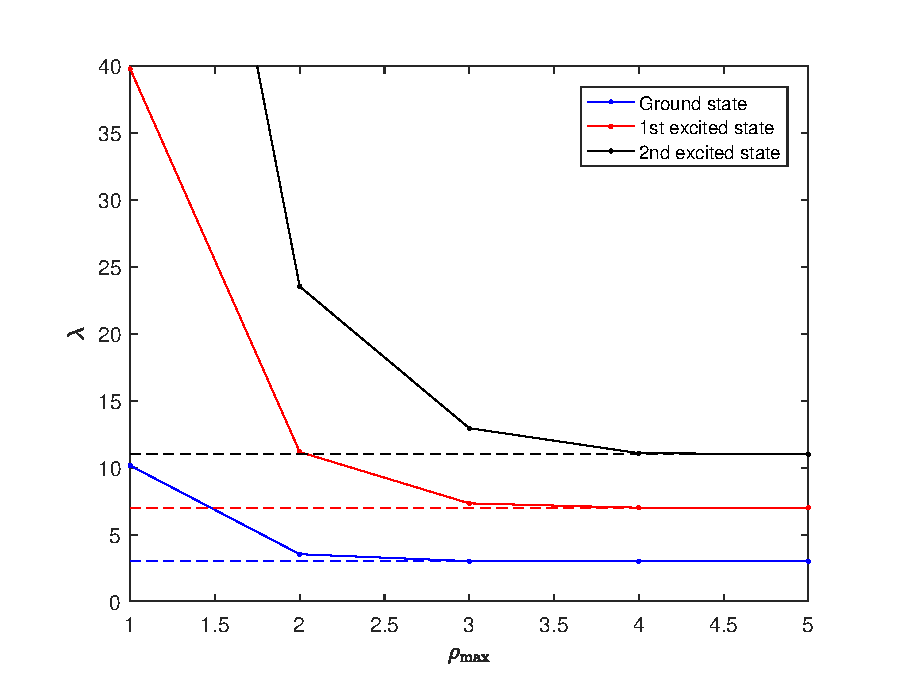
\includegraphics[width=0.7\textwidth]{lambda_rmax.eps}
\caption{Relation between $\rho_{\max}$ and the lowest three eigenvalues of quantum dot with one electron inside a harmonic oscillator potential. Grid spacing $h$ is fixed to be 0.01. Analytical values are given by dashed lines. }
\end{figure}
\begin{table}[tb]
	\centering
	\caption{Relation between different grid number $N$ and the lowest three eigenvalues of quantum dot with one electron inside a harmonic oscillator potential. $\rho_{\max}$ is fixed to be 4. }
	\label{tab:diffN}
	\begin{tabular}{cccc}
		\hline
		\hline
		N   & Ground state & 1st excited state & 2nd excited state \\
		\hline
		10  & 2.9491 & 6.7428 & 10.3971 \\
		20  & 2.9875 & 6.9402 & 10.9154 \\
		40  & 2.9969 & 6.9877 & 11.0383 \\
		80  & 2.9992 & 6.9995 & 11.0687 \\
		100 & 2.9995 & 7.0009 & 11.0724 \\
		Analytical & 3 & 7 & 11 \\
		\hline
		\hline
	\end{tabular}
\end{table}
\par
Now we start to discuss the results of quantum dot with two electrons and Coulomb repulsion. 

	\subsection{Performance comparison of different methods}
	
To test the performances of the cyclic Jacobi and the bisection methods, we use these methods to diagonalize the matrix \ref{eq:matrixse}. 
Treating Eq. \ref{analytical} as a standard benchmark, we adjust the error tolerances in algorithms to reproduce first five eigenvalues deviates smaller than $10^{-5}$ form their analytic values. 
The execution time and speedup for different algorithms and sizes are shown in table \ref{bisectiontab}. 

First of all, we see the speedup of cyclic Jacobi method increases with growing sizes, 
because it cuts off the searching time which is proportional to the number of iterations, as well as the matrix size. 
Generally speaking, the promotion we got from the cyclic Jacobi method is acceptable. 
However, both these Jacobi's methods take a lot of time dealing with the matrix whose size is larger than 1,000.
At that time, the bisection method shows its superiority. 
We see its speedup is super-linear and the execution time is in control as the size growing up to 2,000.
\begin{table}[tb]
\centering
\caption{Execution times and speedups for the classical Jacobi, cyclic Jacobi and bisection method for different inout matrix sizes.}
\label{bisectiontab}
\begin{tabular}{cccccc}
\hline
\hline
Size & Classical Jacobi & \multicolumn{2}{c}{Cyclic Jacobi} & \multicolumn{2}{c}{Bisection Method} \\
 \hline
     & Execution time   & Execution time       & Speedup     & Execution time    & Speedup  \\
     &(ms)   & (ms)      &     &(ms)   &  \\
 \hline
50   & 8.817            & 4.189               & 2.105       & 1.084            & 8.132      \\
100  & 82.845           & 26.696              & 3.103       & 2.819            & 29.393     \\
200  & 1340.239         & 208.239             & 6.436       & 7.845            & 170.833    \\
500  & 35269.687        & 5085.778            & 6.935       & 34.520           & 1021.717   \\
1000 &$\cdots$                  &$\cdots$                     &$\cdots$             & 119.494          &$\cdots$            \\
2000 &$\cdots$                  &$\cdots$                     &$\cdots$             & 418.566          & $\cdots$           \\
\hline
\hline
\end{tabular}
\end{table}
 
	
	\section{Conclusions and outlook}\label{conclude}
	Wait to be filled. 
	
	\section*{Acknowledgments}
	We are grateful for the sincere guidance from Prof. Morten Hjorth-Jensen. 
	
	\nocite{*} 
	\bibliographystyle{plain}
	\bibliography{proj2_ref}
\end{document}